\documentclass[.../Dokumentation.tex]{subfiles}
\begin{document}
\subsection{Fahrzeuge}\label{sec-ita1-cars}
Vor Beginn erster Modellierungsarbeiten wurden zunächst bemaßte Skizzen, 
zu sehen in Abbildung \ref{fig-car-sketch}, angefertigt. 
Hierdurch war es möglich, den ermittelten Platzbedarf der Hardware 
Komponenten abzuschätzen und einen ersten Eindruck der Dimensionen der 
Fahrzeuge zu erhalten.\\
\begin{figure}[H]
    \begin{center}
    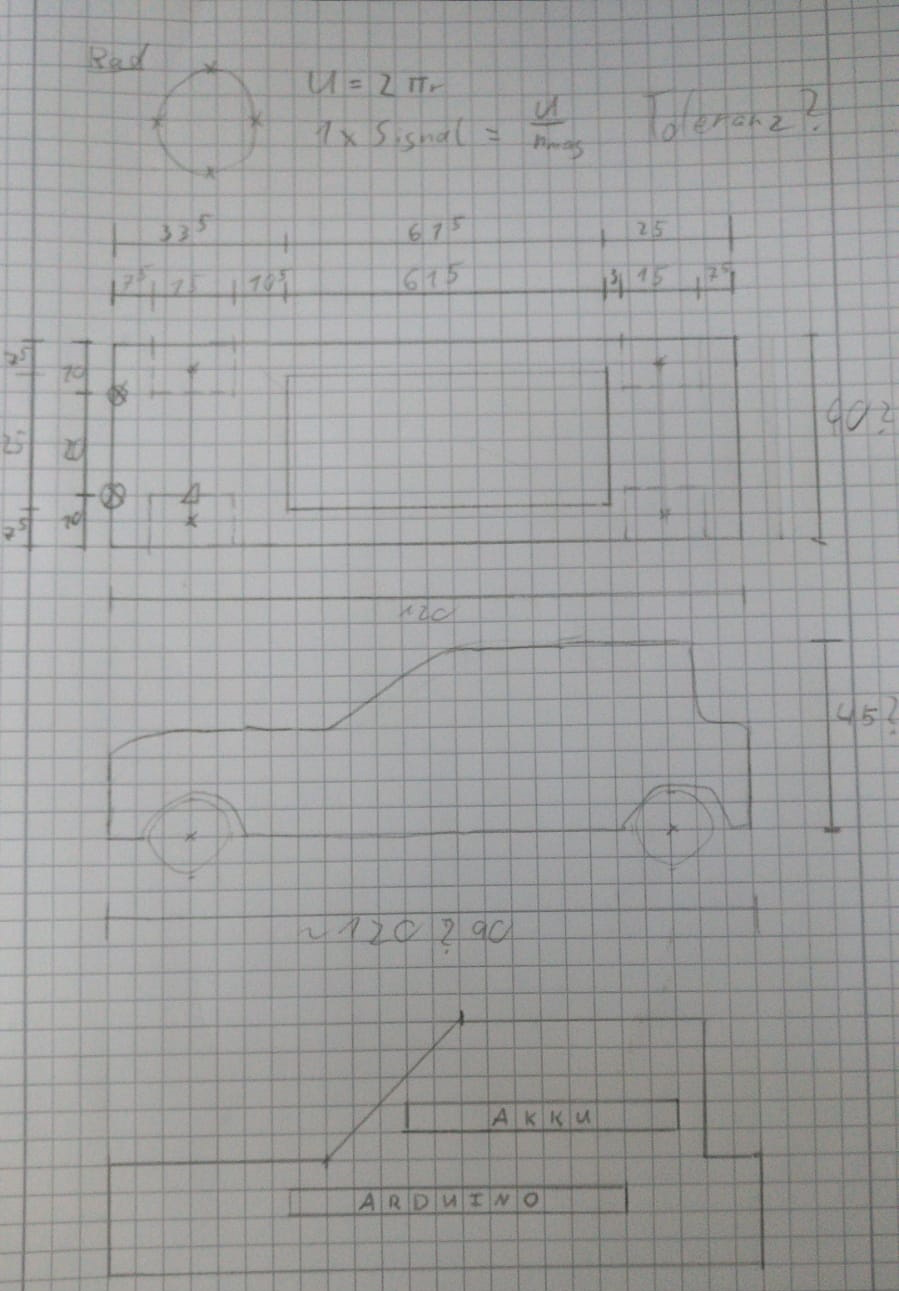
\includegraphics[
        width=0.5\linewidth,
    ]{imgs/car_sketch.jpeg}
    \caption{Erste Skizze eines Fahrzeugs}
    \label{fig-car-sketch}
\end{center}
\end{figure}
\noindent
Bei der eigentlichen Modellierung wurde versucht, zunächst mit so wenig 
Details wie möglich, die grobe Form eines PKW nachzubilden. Hierzu wurde mit 
\textit{Blender} zunächst ein Quader geschaffen, der in seinen Dimensionen 
der Skizze entspricht.\\
Allerdings zeichnete sich bereits bei der Modellierung dieser Rohform ab, 
dass die Arbeiten mit \textit{Blender} in keinem zufriedenstellenden Tempo 
voran schreiten können. Aus diesem Grund wurde die in 
\ref{sec-components-software-model} zur Sprache gekommene Ausweichlösung in 
Form von \textit{SketchUp} für den Rest der Arbeiten verwendet.\\
Der auf diesem Wege geschaffene Quader wurde in seiner Form dahingehend 
manipuliert, dass er äußerlich eher als PKW zu erkennen ist. 
Neben einer angedeuteten Frontsektion mit Motorhaube und abgeschrägter Scheibe 
wurden bereits in diesem Schritt Radkästen und Aussparungen für die später 
benötigten Achsen geschaffen. 
Bei der Dimensionierung der Räder und infolgedessen auch der Radkästen galt 
es zu beachten, dass die verwendeten Magneten ausreichend Platz finden, 
ohne später die strukturelle Integrität des Drucks zu gefährden oder sich so 
nah bei einander befinden, dass vom Hall-Sensor keine einzelnen Magneten 
mehr erkannt werden können.\\
Um den Raum für die elektronischen Komponenten zu schaffen, wurde das Fahrzeug 
horizontal in etwa in der Mitte seiner Höhe in zwei Teilmodelle aufgebrochen.
In sowohl die untere als auch die obere Hälfte wurde nun eine rechteckige 
Aussparung eingearbeitet, die der Skizze aus Abbildung \ref{fig-car-sketch} 
entsprechend ausreichend Platz bietet.
Hierbei galt es zu beachten, Änderungen an den Dimensionen der einen 
Hälfte präzise auf die andere anzuwenden.\\
Die hier beschriebenen Arbeitsschritte sind in den Abbildungen 
\ref{fig-car-side} und \ref{fig-car-slot} zu sehen.
\begin{figure}[H]
\begin{center}
    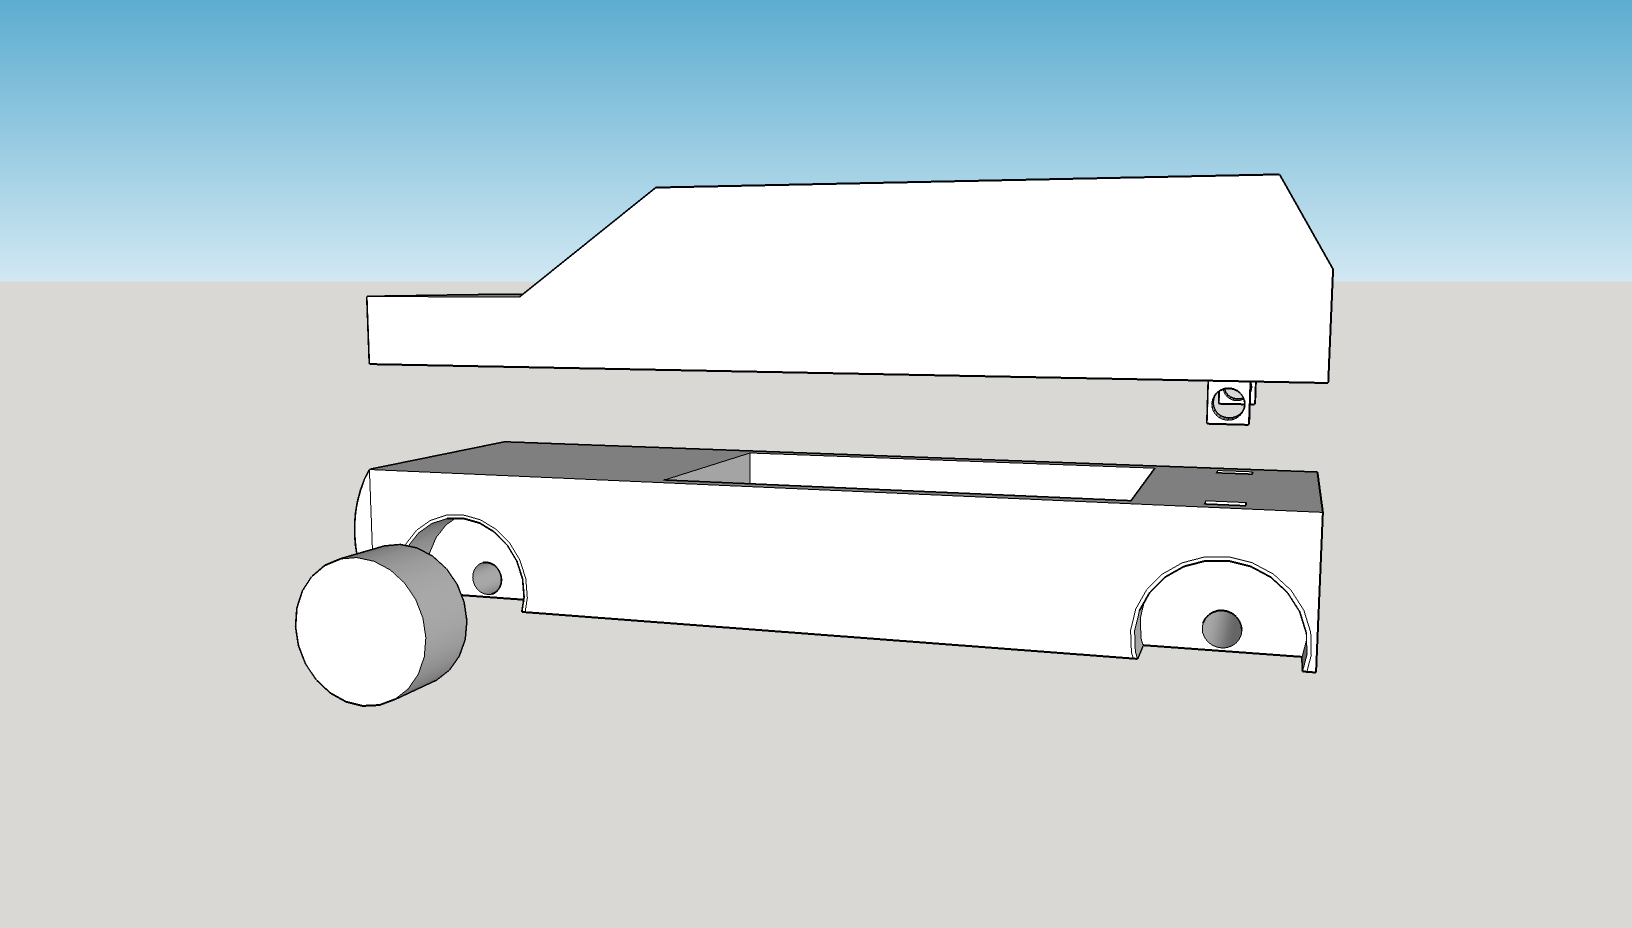
\includegraphics[
        width=0.5\linewidth,
    ]{imgs/car_side.jpg}
    \caption{Seitenansicht des ersten Modells}
    \label{fig-car-side}
\end{center}
\end{figure}
\begin{figure}[H]
\begin{center}
    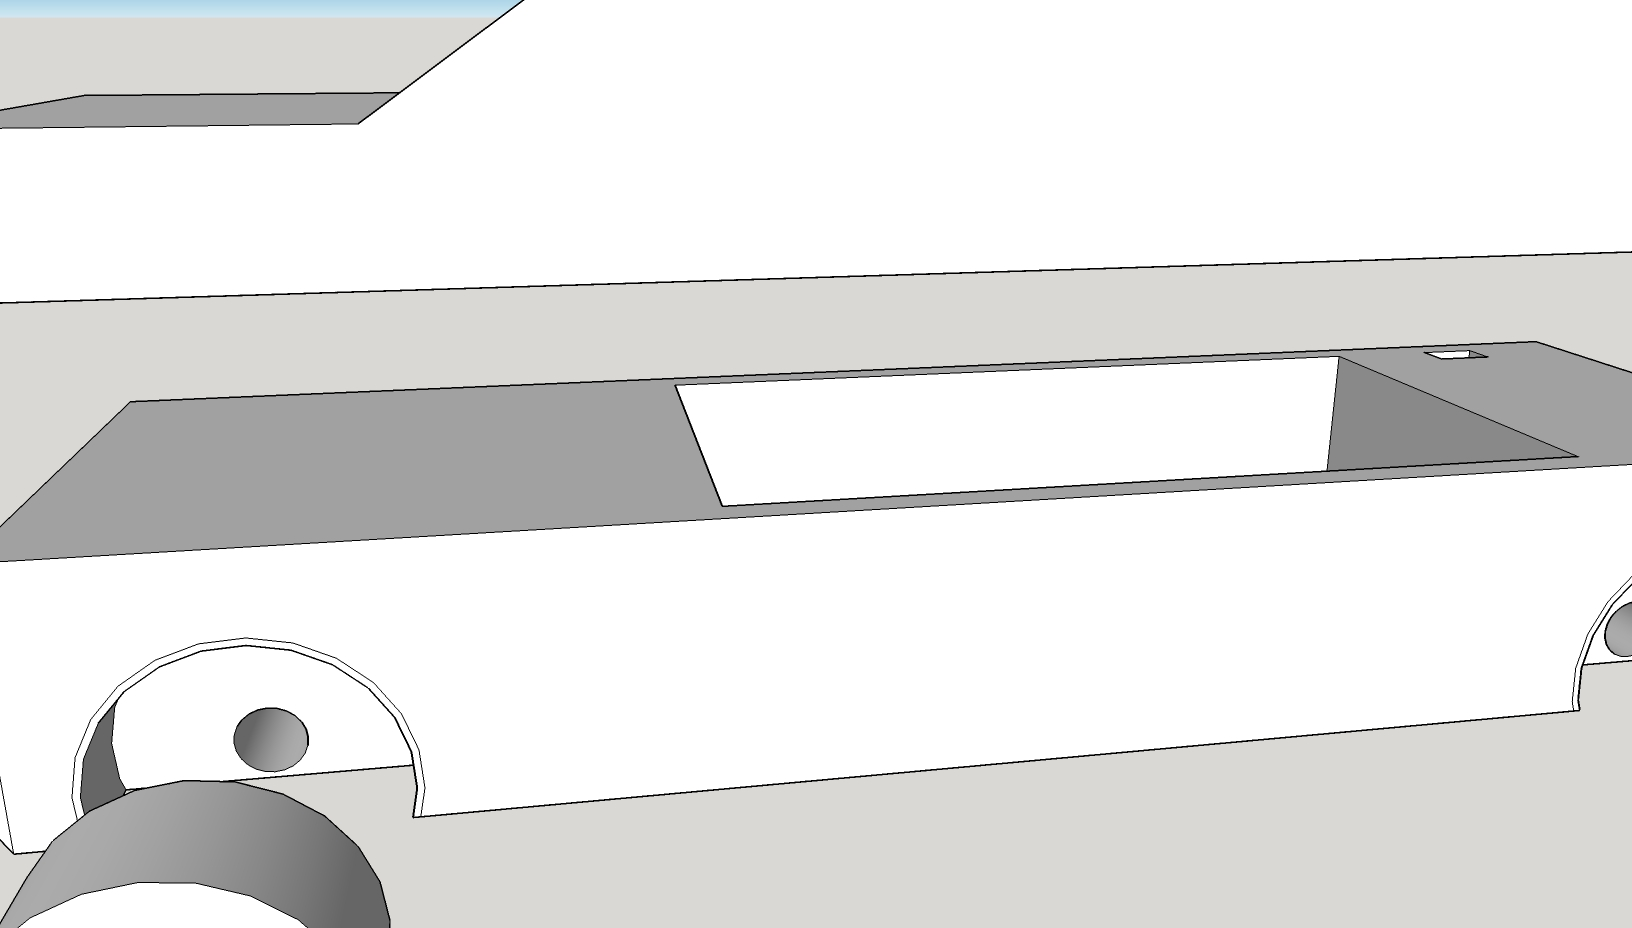
\includegraphics[
        width=0.5\linewidth,
    ]{imgs/car_hardware_slot.jpg}
    \caption{Aussparung im ersten Modell}
    \label{fig-car-slot}
\end{center}
\end{figure}
\noindent
Abbildung \ref{fig-car-side} zeigt weiter einen ersten Ansatz, um beide 
Fahrzeughälften miteinander verbinden und so fixieren zu können. 
In der unteren Hälfte werden Aussparungen vorgesehen, in die entsprechende 
Elemente der oberen eingelassen werden können. Diese zeichnen sich durch eine 
ösenartige Form aus. Somit ist es möglich, entsprechend bemessene Bolzen durch 
beide Hälften zur gleichen Zeit zu führen, um diese zu fixieren.\\
Um zu gewährleisten, dass die aus der Skizze übernommenen Maße 
zufriedenstellend sind, wurde an dieser Stelle mit einem ersten Druck begonnen.
Die in \textit{Cura} verwendeten Einstellungen wurden unter Anleitung 
des \textit{FabLab} Personals an den jeweiligen Drucker angepasst. 
Abbildung \ref{fig-car-firstPrint} zeigt das Ergebnis dieses Drucks.
\begin{figure}[H]
    \begin{center}
        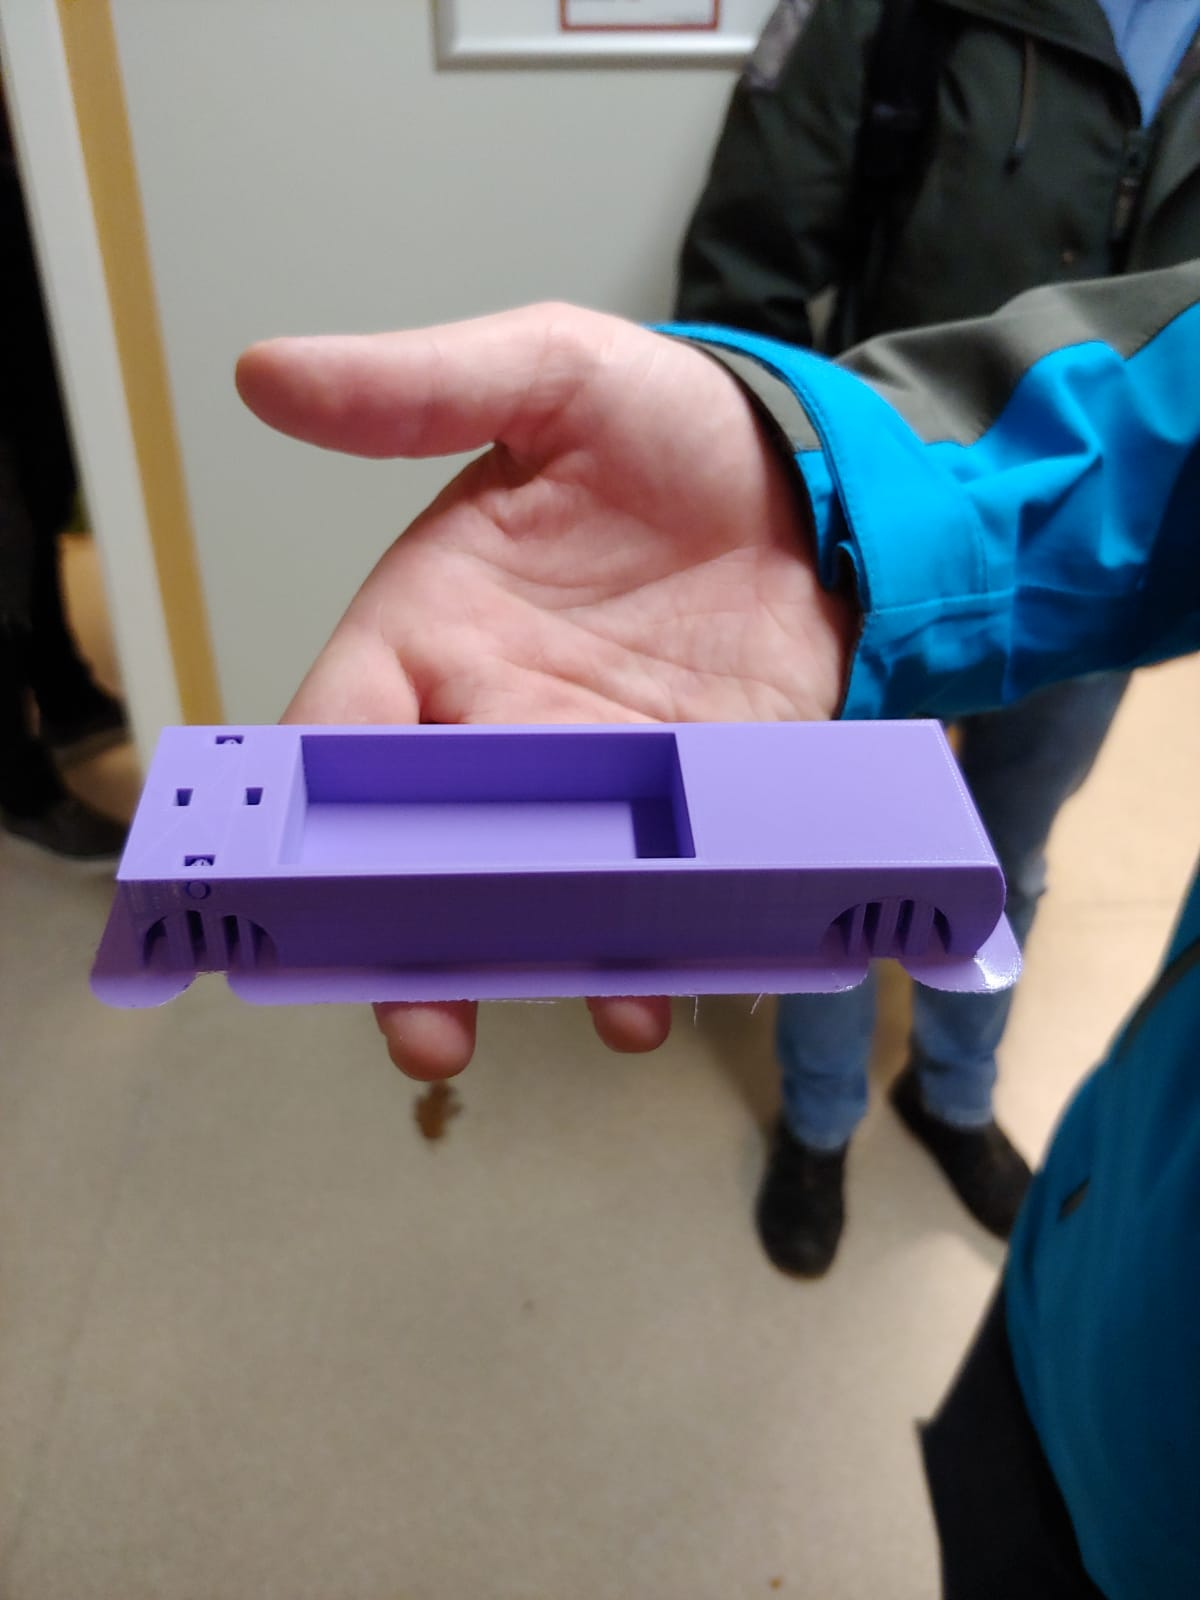
\includegraphics[
            width=0.5\linewidth,
        ]{imgs/car_firstPrint.jpg}
        \caption{Druck des ersten Modells}
        \label{fig-car-firstPrint}
    \end{center}
    \end{figure}
\end{document}